\documentclass{kcc}

% include additional packages you need to use
\usepackage{graphicx}
\usepackage{float}
\usepackage{enumitem}
\usepackage{amsmath}
\usepackage{amssymb}
\usepackage{booktabs}
\usepackage{tabularx}
\usepackage{cite}
\usepackage{listings}
\usepackage{color}

% NanumGothic 및 Times New Roman 기본 폰트 바인딩 (클래스 기본 설정 상속)
\definecolor{codegreen}{rgb}{0,0.6,0}
\definecolor{codegray}{rgb}{0.5,0.5,0.5}
\definecolor{codepurple}{rgb}{0.58,0,0.82}
\definecolor{backcolour}{rgb}{0.96,0.96,0.94}

\lstdefinestyle{mystyle}{
    backgroundcolor=\color{backcolour},   
    commentstyle=\color{codegreen},
    keywordstyle=\color{magenta},
    numberstyle=\tiny\color{codegray},
    stringstyle=\color{codepurple},
    basicstyle=\ttfamily\scriptsize,
    breakatwhitespace=false,         
    breaklines=true,                 
    captionpos=b,                    
    keepspaces=true,                 
    numbers=none,                    
    numbersep=5pt,                  
    showspaces=false,                
    showstringspaces=false,
    showtabs=false,                  
    tabsize=2
}

\lstset{style=mystyle}

\title{메타버스 기술을 활용하여 몰입감이 향상된 오디오-햅틱 인터랙션 리듬게임 구현}
\author{
\vspace{4mm}
경희대학교 컴퓨터공학과 최효석$^{\circ}$\\
\texttt{klasun1072@khu.ac.kr}
\vspace{4mm}
}
\engtitle{Implementation of Audio-Haptic Interaction Rhythm Game with Enhanced Immersion Using Metaverse Technology}
\engauthor{
\ \ \\
\ \ \\
\ \ 
}

\abstract{최근 가상현실(VR) 및 메타버스 기술의 급격한 발전으로 인해 게임 환경에서의 시각 및 청각적 몰입감은 비약적으로 향상되었다. 그러나 기존의 메타버스 콘텐츠는 감각 피드백이 주로 시·청각 영역에 편중되어 있어, 가상 공간 내 개체와 물리적으로 동기화되었다는 실재감(Presence)을 주는 데에는 기술적 한계가 존재한다. 본 연구에서는 가상현실 환경 하에서 실시간 음원 분석과 다차원 햅틱 피드백 기술을 결합하여 시·청·촉각의 다중 감각 동기화를 달성하고 몰입감을 극대화한 VR 리듬게임 시스템을 제안한다. }

\begin{document}
\maketitle

\section{서 론}
최근 VR, AR 및 메타버스 기술의 발전으로 인해 게임에서의 시각적, 청각적인 몰입감은 비약적으로 상승하였다. 하지만 대부분의 게임 콘텐츠는 시각적, 청각적 정보의 전달만을 중점으로 두고 있어 사용자로 하여금 게임 환경에 실제적으로 연결되어 있다는 감각을 주기에는 한계가 존재한다. 또한 시각적, 청각적 정보 이외에 다른 감각적 정보를 느끼지 못하여 몰입감에서 부족한 부분이 필연적으로 존재하게 된다.

다양한 게임 장르들 중에서도 리듬게임은 게임의 음악과 그에 맞춘 행동이 동기화되는 것을 인지하는 과정이 핵심적인 재미 요소이다. 하지만 현재 리듬게임의 경우 화면의 노트(시각적인 영역)와 음악(청각적인 영역)이 동기화되는 것에만 집중하며, 그 외 감각의 동기화에는 집중하지 않는다. 이는 리듬게임에서의 몰입감을 일부 저해하는 요소로 작용하므로, 해당 부분을 보완한 새로운 상호작용이 추가된 게임을 구현하고자 한다.

해당 프로젝트에서는 이를 위해 메타버스 기술 중 하나인 햅틱 인터랙션(Interaction)을 리듬게임 장르에 추가하여 시각, 청각뿐만 아니라 촉각의 동기화까지 구현하고자 한다. 단순히 음원에 따라 지정된 패턴으로 진동이 발생하는 것이 아니라, 음원의 주파수에 따라 메인 멜로디나 날카로운 고음역대 사운드는 햅틱 슈트의 후면부 진동으로, 베이스 드럼 등의 저음역대 비트 성분은 슈트의 전면부 진동으로 분할하여 발생시키고, 각 대역의 진동 변화량에 따라 강도를 동적으로 다르게 전달하는 촉각 시스템을 구현하는 것을 목표로 한다. 이를 통하여 사용자는 리듬게임에서의 음원에 따라 다른 촉각적인 피드백을 느낄 수 있으며, 이를 통해 시각, 청각을 넘어선 촉각에서의 동기화를 통한 몰입감 향상을 기대할 수 있다.

\section{시스템 설계 및 핵심 알고리즘}
제안하는 오디오-햅틱 리듬게임 시스템은 크게 실시간 오디오 분석을 통한 햅틱 신호 처리 파이프라인, 양손 컨트롤러 햅틱 매핑 블록, 3D 트랙상의 노트 동기화 블록으로 구성된다. 전체 모듈의 계층 구조 및 세부 매개변수 사양은 표 \ref{tab:modules}에 요약되어 있다. 또한, 처리 흐름의 직관적 이해를 돕기 위해 실시간 신호 처리 파이프라인을 그림 \ref{fig:pipeline}에 시각화하였다.

\begin{table}[!ht]
\centering
\small
\renewcommand{\arraystretch}{1.4}
\caption{시스템 핵심 모듈 및 하드웨어 사양}
\label{tab:modules}
\begin{tabularx}{\linewidth}{l >{\raggedright\arraybackslash}p{3.8cm} >{\raggedright\arraybackslash}X}
\toprule
{\bfseries 계층/모듈} & {\bfseries 관련 장치 및 도구} & {\bfseries 세부 역할} \\
\midrule
오디오 분석 & Unity Audio Mixer, FFT & 256샘플 분석을 통한 파형 데이터 출력 \\
햅틱 신호 처리 & 대역별 평균필터, Delta 비교 & 대비 승수 $\gamma = 2.5$, 임계값 $\theta_{bass}$, $\theta_{treble}$ 적용 \\
햅틱 공간 매핑 & bHaptics TactSuit X40 / Oculus Touch & 슈트 전후면 그라데이션 매핑 설계 및 컨트롤러 대체 연동 \\
인터랙션 처리 & OVR Camera Rig, XRI & 양손 트래킹, 라인축 동기 회전 및 캘리브레이션 \\
\bottomrule
\end{tabularx}
\end{table}

\begin{figure}[!ht]
\centering
\setlength{\unitlength}{1mm}
\begin{picture}(70,45)
% Boxes
\put(5,35){\framebox(22,8){\scriptsize 오디오 버퍼}}
\put(43,35){\framebox(22,8){\scriptsize FFT (256 Bins)}}
\put(43,20){\framebox(22,8){\scriptsize 대역 평균 계산}}
\put(5,20){\framebox(22,8){\scriptsize Delta 변화량 추적}}
\put(5,5){\framebox(22,8){\scriptsize 대비 및 임계값 필터}}
\put(43,5){\framebox(22,8){\scriptsize 컨트롤러 매핑}}
% Arrows
\put(27,39){\vector(1,0){16}}
\put(54,35){\vector(0,-1){7}}
\put(43,24){\vector(-1,0){16}}
\put(16,20){\vector(0,-1){7}}
\put(27,9){\vector(1,0){16}}
\end{picture}
\caption{실시간 오디오-햅틱 신호 처리 및 매핑 파이프라인}
\label{fig:pipeline}
\end{figure}

\subsection{오디오 주파수 대역 분석}
Unity의 AudioSource.GetSpectrumData()를 사용하여 FFT 결과로 얻은 음원 파형 데이터인 256개의 주파수 배열 $S[i]$에서 각 주파수에 따른 볼륨 값을 구한다. 샘플링 레이트가 44.1kHz일 때, 배열의 한 요소(Bin)의 대역폭은 $44100 / 512 \approx 86.1\text{ Hz}$가 된다.
저음역대의 에너지를 구하기 위해 서브베이스와 베이스 영역에 대응하는 인덱스 0부터 7까지의 대역($0 \sim 688\text{ Hz}$)을 사용한다. 베이스 드럼 등의 비트 성분을 분석하기 위해 해당 대역의 평균 진폭 $A_{bass}$를 계산한다.

\begin{equation}
W_{bass}[i] = 1.0 - \frac{i}{10.0} \quad (0 \le i \le 7)
\end{equation}
\begin{equation}
A_{bass} = \frac{1}{8} \sum_{i=0}^{7} (S[i] \cdot W_{bass}[i])
\end{equation}

고음역대의 에너지를 구하기 위해 메인 보컬과 일렉트릭 신디사이저 음을 포함하는 주파수 대역($1722 \sim 5166\text{ Hz}$)에 해당하는 인덱스 20부터 60까지의 구간에서 해당 대역의 평균 진폭 $A_{treble}$을 계산한다.

\begin{equation}
A_{treble} = \frac{1}{41} \sum_{i=20}^{60} S[i]
\end{equation}

\subsection{Delta 추적 및 대비 강조(Contrast) 햅틱 알고리즘}
단순히 오디오의 실시간 볼륨 총합을 진동 세기로 매핑할 경우 입체감을 전달하기에는 부족하다는 한계가 존재한다. 따라서 이를 해결하기 위하여 이전 프레임의 대역별 평균 진폭과의 차이값(Delta)인 델타 값($\Delta$)을 실시간으로 계산하는 알고리즘을 사용한다.

현재 프레임 $t$에서의 변화량 $\Delta_{bass}$와 $\Delta_{treble}$은 다음과 같이 정의된다.

\begin{equation}
\Delta_{bass} = A_{bass, t} - A_{bass, t-1}
\end{equation}
\begin{equation}
\Delta_{treble} = A_{treble, t} - A_{treble, t-1}
\end{equation}

비트의 순간적인 변화량을 잡는 델타 계산과 통합하여 강하고 약한 음의 세기 편차를 늘려 사용자의 체감을 극대화하기 위해 각 음역대 간 대비(Contrast) 상수를 지정하고, 최종 값 계산 시 이를 적용한다. 델타 값이 지정된 임계값(Threshold) $\theta$를 초과하여 비트가 감지될 때, 출력되는 최종 햅틱 강도 $V$는 평균 진폭 $A$와 햅틱 감도 계수 $\mu$의 곱에 대비(Contrast) 상수 $\gamma$를 거듭제곱하여 연산한다.

\begin{equation}
V_{bass} = \begin{cases} (A_{bass, t} \cdot \mu_{bass})^\gamma & (\Delta_{bass} > \theta_{bass}) \\ 0 & (\Delta_{bass} \le \theta_{bass}) \end{cases}
\end{equation}
\begin{equation}
V_{treble} = \begin{cases} (A_{treble, t} \cdot \mu_{treble})^\gamma & (\Delta_{treble} > \theta_{treble}) \\ 0 & (\Delta_{treble} \le \theta_{treble}) \end{cases}
\end{equation}

여기서 $\mu_{bass}$와 $\mu_{treble}$은 각 음역대의 햅틱 감도 계수이며, 대비(Contrast) 상수 $\gamma$는 $2.5$로 설정되어 약한 진폭 성분은 더 감소시키고 강한 진폭 성분은 더 증가시켜 타격감의 대비를 극대화한다. 연산된 $V_{bass}$와 $V_{treble}$ 값은 최종적으로 컨트롤러의 진동 세기 입력 범위인 $[0, 1]$ 범위로 제한된다.

이러한 델타 변화량 추적 및 대비 알고리즘의 결합을 통해, 각 리듬의 음역대에 따라 선명한 오디오-햅틱 입체감을 실현할 수 있다.

\subsection{햅틱 슈트 공간 매핑}
최종 계산된 $V_{bass}$와 $V_{treble}$ 세기 값은 TactSuit X40 웨어러블 햅틱 의복의 전후면 40개 진동 모터에 실시간 공간 매핑되도록 설계되었다. 

저주파(베이스)의 무게감을 흉부에 표현하기 위해 앞면 20개 모터(인덱스 0~19) 전체에 동일한 $V_{bass}$ 강도로 진동 신호를 매핑하였다. 반대로 고주파(트레블)의 선명하고 높은 타격감은 뒷면 20개 모터(인덱스 20~39) 전체에 동일한 $V_{treble}$ 강도로 진동 신호를 매핑하였다. 진동 시점마다 매 프레임 기준 햅틱 드라이버 API를 통해 전후면의 진동 출력값이 전송되도록 구현하였다.

단, 본 연구의 최종 통합 단계에서 하드웨어 SDK 호환 및 연동 테스트 환경의 한계로 인해, 설계 및 구현된 슈트 제어 로직을 가상현실 양손 컨트롤러의 좌우 진동 모터(우측: 저음역 $V_{bass}$, 좌측: 고음역 $V_{treble}$)에 매핑하여 진동을 구현하는 것으로 대체하였다.

\section{시스템 구현}
\subsection{가상현실 리듬게임 클라이언트 및 노트 제어}
VR 리듬게임 클라이언트는 Unity 엔진으로 개발하였으며 Meta Quest 헤드셋과의 연동을 위해 OpenXR 및 XR Interaction Toolkit 인터랙션 프레임워크를 기반으로 구축하였다. 본 게임은 3차원 트랙 상에서 다가오는 3종의 노트를 사용자가 알맞게 컨트롤러로 타격, 유지, 회전하며 플레이하는 메커니즘을 지닌다.

가상현실 공간상에 실시간으로 생성되는 노트들은 상속 구조를 갖는다. NoteSpawner를 통해 생성되는 모든 노트 유형은 공통으로 \texttt{BaseNote} 추상 클래스를 상속하며, 이를 기반으로 충돌 체크와 판정선 접근 물리 동작이 제어된다.

\begin{itemize}[itemsep=0pt,parsep=0pt]
  \item \textbf{PunchNote(일반 노트)}: 플레이어가 판정 영역 도달 시점에 컨트롤러 혹은 손을 위치시켜 노트와 접촉을 발생시키면 점수를 얻는다.
  \item \textbf{HoldNote(홀드 노트)}: 판정 지점에 도달한 순간부터 일정 시간 동안 지정된 터치 영역 내에 양손의 위치를 고정 및 유지시키면 점수를 얻는다.
  \item \textbf{RotateNote(회전 노트)}: 노트가 다가오는 동안 플레이어가 트랙 방향과 각도량을 맞추어 회전 인터랙션을 수행하면 라인이 회전하며 점수를 얻는다.
\end{itemize}

특히, 차별화된 플레이 경험을 위해 모바일 리듬게임 Rotaeno에서 영감을 받은 \textbf{라인 회전 시스템}을 구현하였다. 회전 노트를 정상적으로 처리하면, 노트가 내려오는 트랙 라인의 중심축 자체가 해당 방향 및 각도만큼 실시간으로 회전한다. 이는 단순 직선 궤적을 벗어나 사용자가 판정 영역을 추적하여 플레이하도록 하여 역동성을 높인다. 또한 가상 공간 내에서 위치 이동 및 상하 높이 차이에 대한 조정을 위해 버튼 입력으로 사용자의 시선과 중심점을 기준으로 판정 영역과 UI를 재정렬하는 \textbf{캘리브레이션 시스템}을 구축하였다.

\subsection{양손 상대 위치 기반 트랙 회전 알고리즘}
트랙 회전 기능은 플레이어가 쥐고 있는 두 가상현실 컨트롤러의 상대적인 위치와 각도 변화를 실시간으로 계산하여 화면 중앙의 트랙을 회전시키는 기능이다. 

왼쪽 컨트롤러의 위치 $P_L(x_L, y_L, z_L)$과 오른쪽 컨트롤러의 위치 $P_R(x_R, y_R, z_R)$의 좌표 차이를 구한 뒤, 두 컨트롤러가 이루는 기울기 각도 $\theta_{hand}$를 다음 식 (9)와 같이 아크탄젠트(Atan2) 함수를 사용하여 계산한다.

\begin{equation}
\theta_{hand} = \text{atan2}(y_R - y_L, x_R - x_L) \cdot \text{Rad2Deg}
\end{equation}

이렇게 계산된 양손의 각도 변화 속도가 미리 설정한 기준값($180^\circ/\text{s}$)보다 빠를 때 메인 트랙에 회전 효과가 적용되도록 구현하였다. 

이때 Unity 엔진의 부모-자식 관계를 활용하여, 생성된 노트들을 트랙 오브젝트의 자식 객체로 등록하였다. 이 덕분에 트랙이 회전할 때 노트들도 별도의 복잡한 좌표 변환 연산식 없이 부모인 트랙의 움직임을 따라 자연스럽게 함께 회전하며 이동하게 된다. 

플레이어는 회전노트를 입력시 노트의 기준 라인이 회전하여 판정영역이 지속적으로 회전해 그에 맞춰 노트를 타격해야 하므로 기존의 단순한 리듬게임에 비해 훨씬 역동적이고 몰입감 있는 조작감을 느끼게 된다.


\subsection{실시간 캘리브레이션 및 횡방향 정렬}
HMD 착용자의 실제 서 있는 키나 초기 위치의 이탈로 발생할 수 있는 판정 영역 불일치를 방지하기 위해 Calibration 시스템을 구현하였다. 사용자가 오른쪽 컨트롤러의 보조 버튼을 누르는 즉시 헤드셋 중심 앵커의 XZ 수평 좌표를 기준으로 트랙의 중심축을 Snap하여 위치를 정렬하고, 시선 방향에 맞추어 트랙 전체의 방향을 정렬함으로써 위치를 정렬하고, 위치를 설정하기 위해 재시작하는 불편함을 제거하였다.

\subsection{UI 및 씬 매니지먼트 구현}
가상현실 사용자 경험을 보장하기 위하여 게임 루프의 전 과정을 유기적으로 묶는 UI Scene 체계를 설계하였다.
\begin{itemize}[itemsep=0pt,parsep=0pt]
  \item \textbf{MainMenuUI}: 게임을 처음 구동했을 때 플레이 영역 전면에 등장하는 3D 메인 메뉴이다. 사용자의 컨트롤러를 이용한 Ray Casting 포인터를 통해 곡 선택 화면으로 전환하거나, 게임을 종료할 수 있다.
  \item \textbf{SongSelectUI}: 사용자가 플레이할 음원을 미리 선택하고 BPM와 곡 길이를 확인할 수 있는 창이다.
  \item \textbf{PauseUI}: 게임 도중 메뉴 버튼을 눌렀을 때 등장하며, 일시정지 시 오디오 재생 버퍼를 멈춤과 동시에 생성되어 다가오는 모든 노트와 시각 파티클 이펙트를 
비활성화한다. 해당 창에서 Song Select 창으로 다시 이동하거나, 게임을 다시 재개할 수 있다.
  \item \textbf{ResultUI}: 게임 종료 후 점수, 최대 콤보, 정확도와 같은 플레이 성과를 출력한다.
\end{itemize}

\subsection{점수 계산 및 판정 시스템}
유저가 노트를 타격했을 때 정확도를 평가하는 판정 시스템을 구현하였다.
노트 타격 시 타겟 판정선(HitArea)과의 거리 오차를 계산하여 총 4개의 판정으로 분류한다. 노트의 접근 속도는 배속 설정(도달 시간) 로직에 의해 등속으로 운동하므로 판정 구역과의 거리는 시간적 오차 $\Delta t_{error}$로 매핑된다.
\begin{itemize}[itemsep=0pt,parsep=0pt]
  \item \textbf{Perfect}: 거리 $\le 0.35\text{ m}$ ($\Delta t_{error} \le 35\text{ms}$ 대응, 100점 지급, 콤보 증가)
  \item \textbf{Great}: $0.35\text{ m} < \text{거리} \le 0.70\text{ m}$ ($\Delta t_{error} \le 70\text{ms}$ 대응, 80점 지급, 콤보 증가)
  \item \textbf{Good}: $0.70\text{ m} < \text{거리} \le 1.20\text{ m}$ ($\Delta t_{error} \le 120\text{ms}$ 대응, 50점 지급, 콤보 유지)
  \item \textbf{Bad}: 거리 $> 1.20\text{ m}$ ($120\text{ms}$ 초과 대응, 20점 지급, 콤보 리셋)
  \item \textbf{Miss}: 판정 영역 통과 및 타격 실패 시 (점수 없음, 콤보 리셋)
\end{itemize}
판정 결과는 \texttt{ScoreManager}를 통해 콤보 수와 누적 정확도로 집계되며, \texttt{JudgementText} 컴포넌트를 통해 3D 텍스트 형태로 일정시간동안 출력되었다가 사라지도록 연출하였다.



\subsection{핵심 C\# 스크립트 구현 코드}
구현된 시스템 중 FFT를 이용한 음원 파형 데이터 출력,  VR 컨트롤러 햅틱 매핑, 그리고 상호작용 관련 핵심 소스코드는 다음 리스트 \ref{lst:haptic}부터 리스트 \ref{lst:beatmap}과 같다.

\begin{lstlisting}[language=C++, caption=AudioReactionSystems.cs FFT 이용 파형 데이터 분석 및 Delta+Contrast 로직, label=lst:haptic]
// AudioReactionSystems.cs
void Update() {
    if (audioSource == null) return;
    audioSource.GetSpectrumData(spectrum, 0, FFTWindow.BlackmanHarris);

    float bassSum = 0f;
    for (int i = 0; i <= 7; i++) {
        float weight = 1.0f - (i / 10.0f);
        bassSum += spectrum[i] * weight;
    }
    float bassAvg = bassSum / 8f;

    float trebleSum = 0f;
    for (int i = 20; i <= 60; i++) {
        trebleSum += spectrum[i];
    }
    float trebleAvg = trebleSum / 41f;

    float bassDelta = bassAvg - lastBassAvg;
    float trebleDelta = trebleAvg - lastTrebleAvg;

    float finalBass = 0f;
    if (bassDelta > bassThreshold) {
        float scaledBass = Mathf.Clamp01(bassAvg * bassSensitivity);
        finalBass = Mathf.Pow(scaledBass, depthContrast);
    }

    float finalTreble = 0f;
    if (trebleDelta > trebleThreshold) {
        float scaledTreble = Mathf.Clamp01(trebleAvg * trebleSensitivity);
        finalTreble = Mathf.Pow(scaledTreble, depthContrast);
    }

    FinalBass = Mathf.Clamp01(finalBass);
    FinalTreble = Mathf.Clamp01(finalTreble);

    lastBassAvg = bassAvg;
    lastTrebleAvg = trebleAvg;
}
\end{lstlisting}

\begin{lstlisting}[language=C++, caption=BhapticsAudioHaptic.cs 햅틱 수트 음역대에 따른 진동 매핑, label=lst:bhaptics]
// BhapticsAudioHaptic.cs
void Update() {
    if (!enableBhaptics || audioReaction == null || !BhapticsSDK2.IsInitialized) return;
    if (Time.time - lastUpdateTime < updateInterval) return;
    lastUpdateTime = Time.time;

    float bass = audioReaction.FinalBass;
    float treble = audioReaction.FinalTreble;
    for (int i = 0; i < vestMotors.Length; i++) vestMotors[i] = 0;

    if (bass > 0f) {
        int val = Mathf.Clamp((int)(bass * vestIntensityMultiplier * 100f), 1, 100);
        for (int i = 0; i < 20; i++) {
            vestMotors[i] = val;
        }
    }
    if (treble > 0f) {
        int val = Mathf.Clamp((int)(treble * forearmIntensityMultiplier * 100f), 1, 100);
        for (int i = 20; i < 40; i++) {
            vestMotors[i] = val;
        }
    }
    BhapticsLibrary.PlayMotors((int)PositionType.Vest, vestMotors, vestDurationMs);
}
\end{lstlisting}

\begin{lstlisting}[language=C++, caption=TrackManager.cs RotateNote 작동에 따른 라인 회전, label=lst:track]
// TrackManager.cs
void UpdateTrackRotation() {
    if (leftController != null && rightController != null) {
        Vector3 handDirection = rightController.position - leftController.position;
        float rawAngle = Mathf.Atan2(handDirection.y, handDirection.x) * Mathf.Rad2Deg * rotationSensitivity;
        float deltaAngle = Mathf.DeltaAngle(lastHandAngle, rawAngle);
        float rawVelocity = deltaAngle / Time.deltaTime;
        lastHandAngle = rawAngle;

        CurrentAngularVelocity = Mathf.Lerp(CurrentAngularVelocity, rawVelocity, Time.deltaTime * 35f);
        CurrentHandAngle = rawAngle;

        Quaternion targetRotation = initialRotation * Quaternion.Euler(0, 0, TotalTrackRotation);
        transform.rotation = Quaternion.Lerp(transform.rotation, targetRotation, Time.deltaTime * rotationSmoothSpeed);
    }
}
\end{lstlisting}

\begin{lstlisting}[language=C++, caption=HeightCalibrator.cs 사용자 기준 수직 수평 정렬, label=lst:calib]
// HeightCalibrator.cs
public void CalibrateHeight() {
    if (centerEyeAnchor == null || targetTrack == null) return;
    TrackManager trackManager = targetTrack.GetComponent<TrackManager>();
    if (trackManager != null) {
        trackManager.AlignTrackToPlayer();
    }
    float targetHeight = centerEyeAnchor.position.y + heightOffset;
    if (calibrationCoroutine != null) StopCoroutine(calibrationCoroutine);
    calibrationCoroutine = StartCoroutine(CalibrateRoutine(targetHeight));
}
\end{lstlisting}



\begin{lstlisting}[language=C++, caption=HoldNote.cs 롱노트 양손 홀드 로직, label=lst:hold]
// HoldNote.cs
protected override void Update() {
    base.Update();
    if (isJudged || !holdPhaseStarted) return;

    holdPhaseElapsed += Time.deltaTime;
    float currentLaserLength = laserLengthCached - (speed * holdPhaseElapsed);
    currentLaserLength = Mathf.Max(0f, currentLaserLength);
    if (visualObj != null) {
        visualObj.transform.localScale = new Vector3(1f, currentLaserLength * 0.5f, 1f);
        visualObj.transform.localPosition = new Vector3(0f, 0f, -currentLaserLength * 0.5f);
    }

    bool leftGuarding = Vector3.Distance(transform.position, TrackManager.Instance.leftController.position) <= 0.8f;
    bool rightGuarding = Vector3.Distance(transform.position, TrackManager.Instance.rightController.position) <= 0.8f;

    if (leftGuarding && rightGuarding) {
        actualHoldDuration += Time.deltaTime;
        ProcessHolding();
    }
    if (holdPhaseElapsed >= holdDurationSeconds) JudgeAndDestroy();
}
\end{lstlisting}

\begin{lstlisting}[language=C++, caption=RotateNote.cs 회전 노트 판정 및 각도/속도 조건 추적, label=lst:rotate]
// RotateNote.cs
void CheckSnapAction(float currentDistance) {
    float currentHandAngle = TrackManager.Instance.CurrentHandAngle;
    float velocity = TrackManager.Instance.CurrentAngularVelocity;
    float velocityThreshold = TrackManager.Instance.snapVelocityThreshold;
    float rotatedAmount = Mathf.DeltaAngle(initialHandAngle, currentHandAngle);

    bool isCorrectDirection = (targetAngle > 0 && rotatedAmount > 2f) || (targetAngle < 0 && rotatedAmount < -2f);
    bool isVelocityDirectionCorrect = (targetAngle > 0 && velocity > 0) || (targetAngle < 0 && velocity < 0);
    float minRotationRequired = Mathf.Max(25f, Mathf.Abs(targetAngle) * 0.65f);

    if (isCorrectDirection && isVelocityDirectionCorrect) {
        if (Mathf.Abs(rotatedAmount) >= minRotationRequired && Mathf.Abs(velocity) >= velocityThreshold) {
            Success();
        }
    }
}
\end{lstlisting}

\begin{lstlisting}[language=C++, caption=BeatmapData.cs CSV 텍스트 파싱 및 정렬, label=lst:beatmap]
// BeatmapData.cs
public void ParseCsvToNotes() {
    if (string.IsNullOrEmpty(rawCsvData)) return;
    string[] lines = rawCsvData.Split(new[] { '\n', '\r' }, StringSplitOptions.RemoveEmptyEntries);
    List<NoteData> parsedNotes = new List<NoteData>();
    foreach (string rawLine in lines) {
        string line = rawLine.Trim();
        if (line.StartsWith("#") || line.StartsWith("//")) continue;
        string[] tokens = line.Split(',');
        if (tokens.Length < 3) continue;

        NoteData note = new NoteData { useBeat = true };
        note.beat = float.Parse(tokens[0]);
        note.laneIndex = int.Parse(tokens[1]);
        string typeStr = tokens[2].Trim().ToLower();
        if (typeStr.StartsWith("p")) note.type = NoteType.Punch;
        else if (typeStr.StartsWith("r")) {
            note.type = NoteType.Rotate;
            note.targetAngle = tokens.Length >= 4 ? float.Parse(tokens[3]) : 90f;
        } else if (typeStr.StartsWith("h")) {
            note.type = NoteType.Hold;
            note.duration = tokens.Length >= 4 ? float.Parse(tokens[3]) : 1f;
        }
        parsedNotes.Add(note);
    }
    notes = parsedNotes;
    RecalculateNoteTimes();
}
\end{lstlisting}

\subsection{웹 기반 채보 저작 도구}
채보 제작의 편의성을 높이기 위해 AI를 이용하여 HTML 기반의 채보 에디터(\texttt{BeatmapEditor.html})를 개발하였다. 이 에디터는 로컬 음악 파일을 불러와 음원을 파악한 후 노트를 정확한 박자 타이밍에 배치할 수 있도록 4분음표, 8분음표, 16분음표, 32분음표 단위로 박자를 쪼개어 편집 화면의 타임라인에 기준선을 렌더링한다.

사용자는 음원을 재생하면서 타임라인 위에서 키보드 단축키를 눌러 실시간으로 각 노트를 작성할 수 있으며 마우스 드래그를 이용해 노트 배치 시점을 박자 단위로 이동 및 조정할 수 있다. 제작 완료된 채보는 CSV 형태로 인코딩되어 텍스트 영역에 표시되며 복사 기능을 이용하여 클립보드로 추출할 수 있다. 

해당 과정을 통해 추출한 CSV 데이터는 Unity 에디터 상에서 Import 과정을 통해 리듬게임 노트 생성 및 관리를 위한 ScriptableObject으로 변환되고 플레이 시 해당 오브젝트에 입력된 데이터에 따라 노트가 출력되게 된다.

\section{시스템 구동 및 사용자 인터페이스}
구현된 가상현실 리듬게임 시스템의 실제 플레이 화면과 사용자 인터페이스(UI) 구성은 다음과 같다.

\subsection{게임 시작 및 메인 메뉴}
사용자가 HMD를 착용한 후 게임을 처음 구동하면 플레이 영역 전면에 메인 메뉴 화면이 등장한다. 플레이어는 VR 컨트롤러에서 발사되는 Ray Casting 포인터를 활용하여 메뉴 및 난이도를 선택할 수 있으며, 이어서 곡 선택 화면으로 전환된다. 메인 메뉴 화면의 구동 모습은 그림 \ref{fig:main_menu}에 수록되어 있다.

\begin{figure}[!ht]
\centering
\begin{minipage}[b]{0.48\linewidth}
  \centering
  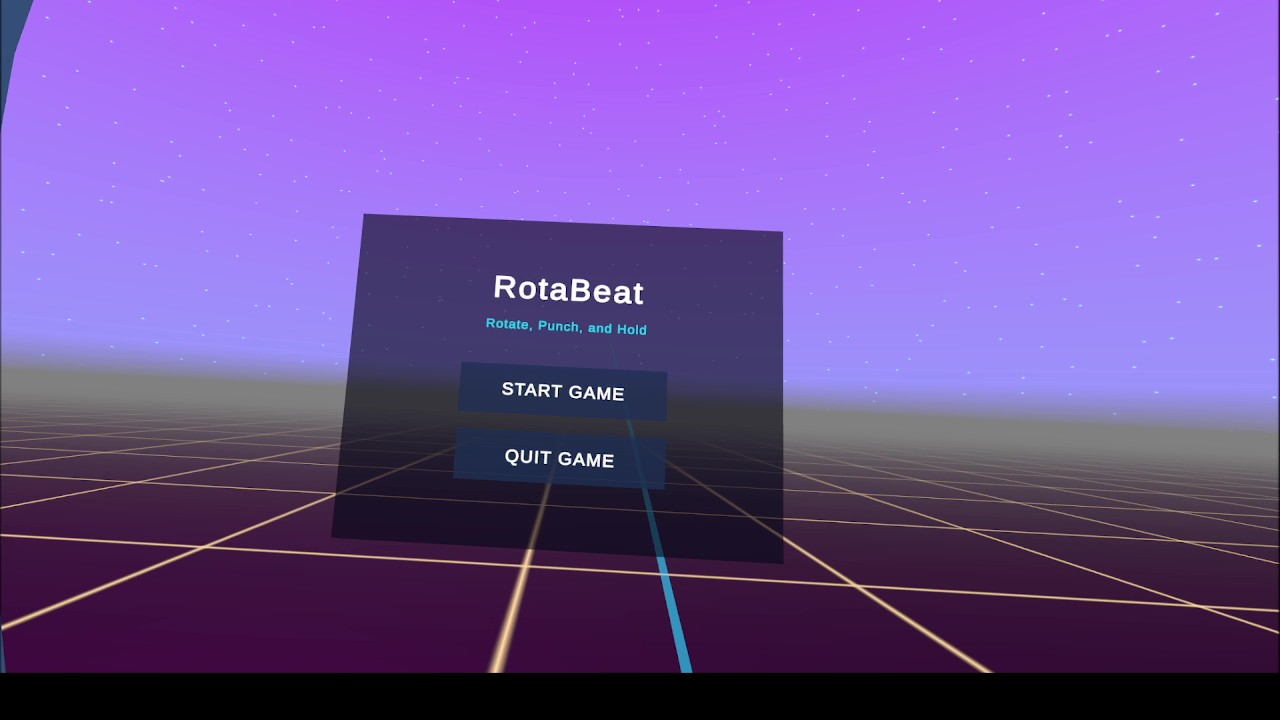
\includegraphics[width=\linewidth]{MainMenuUI.jpg}
  \centering{(a) 메인 메뉴}
\end{minipage}
\hfill
\begin{minipage}[b]{0.48\linewidth}
  \centering
  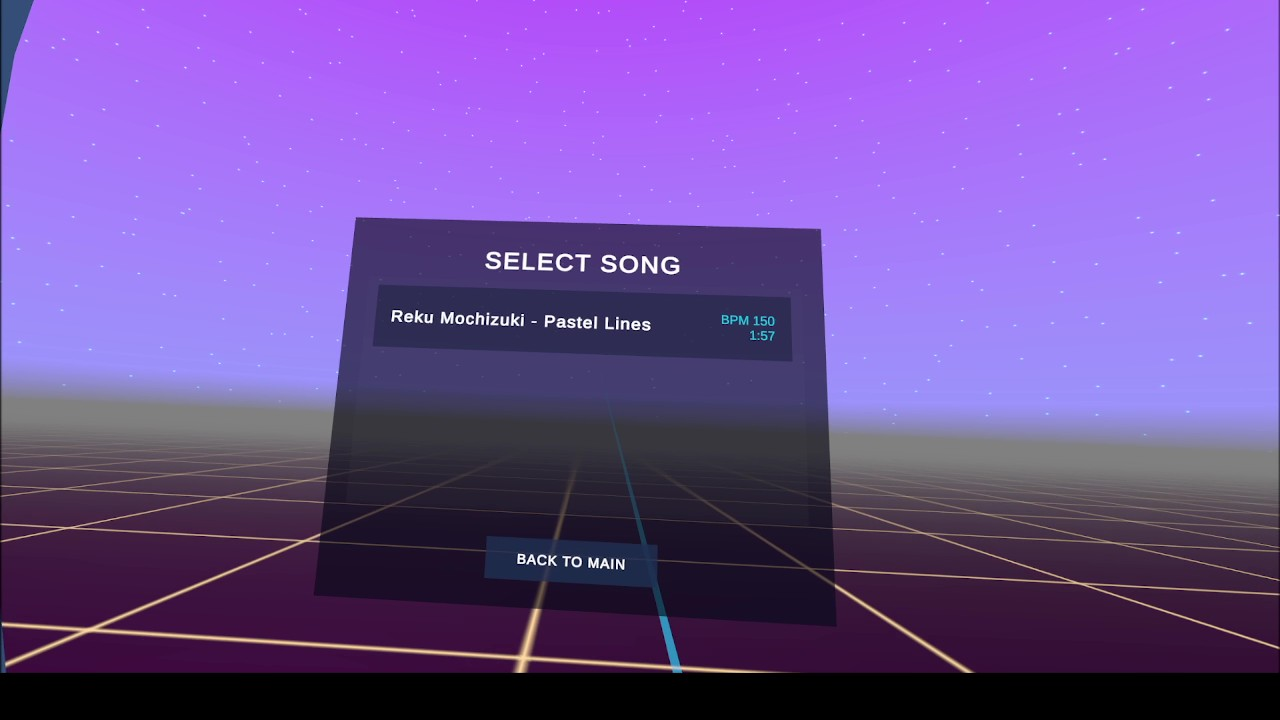
\includegraphics[width=\linewidth]{SongSelectUI.jpg}
  \centering{(b) 곡 선택 화면}
\end{minipage}
\caption{Curved Canvas 형태의 메인 메뉴 및 곡 선택 화면}
\label{fig:main_menu}
\end{figure}

\subsection{인게임 플레이 및 인터랙션}
곡 선택 완료 후 게임이 시작되면 사용자는 3차원 트랙 상에서 자신을 향해 내려오는 3종의 노트를 타격하게 된다. 양손 컨트롤러의 실시간 위치와 회전을 기준으로 일반 노트(PunchNote) 타격 및 홀드 노트(HoldNote) 유지를 수행한다. 특히 회전 노트(RotateNote)의 스냅 액션에 성공할 경우, 그림 \ref{fig:play_screen}과 같이 트랙 전체가 양손의 각도 변화에 맞추어 실시간으로 회전하며, 판정 텍스트가 출력된다.


\begin{figure}[!ht]
\centering
\begin{minipage}[b]{0.48\linewidth}
  \centering
  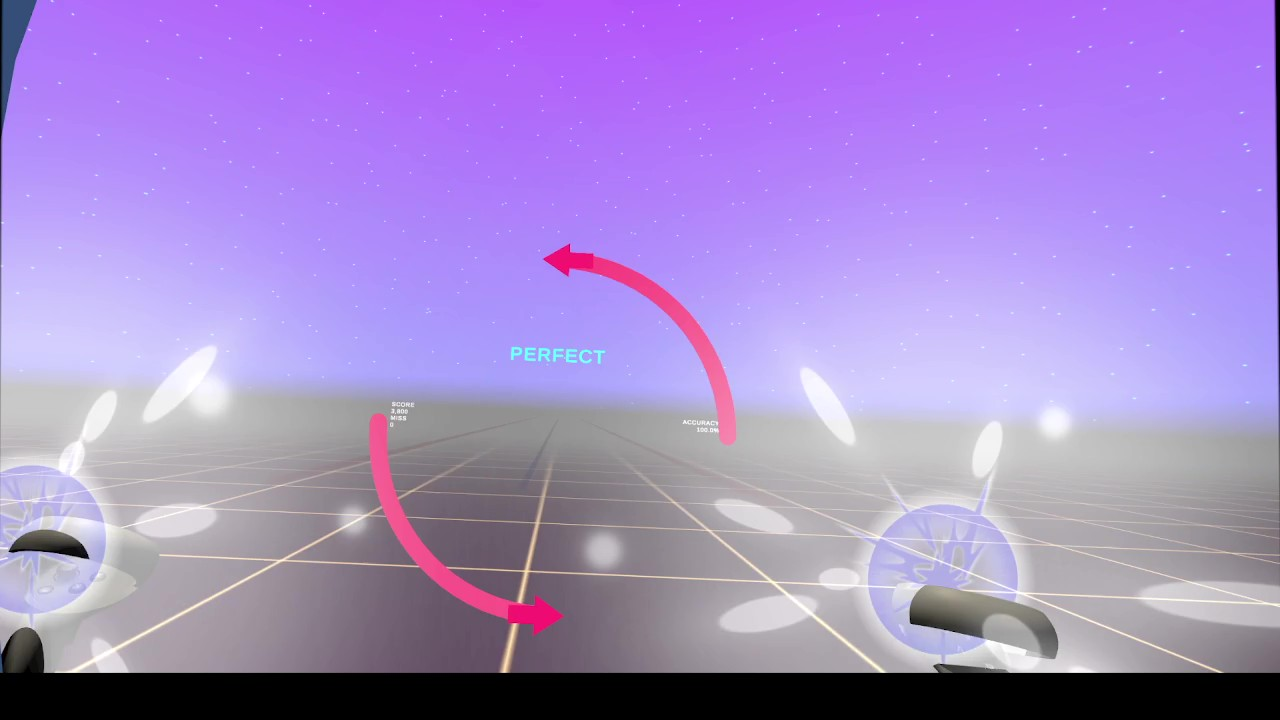
\includegraphics[width=\linewidth]{RotatePrev.jpg}
  \centering{(a) 회전 전}
\end{minipage}
\hfill
\begin{minipage}[b]{0.48\linewidth}
  \centering
  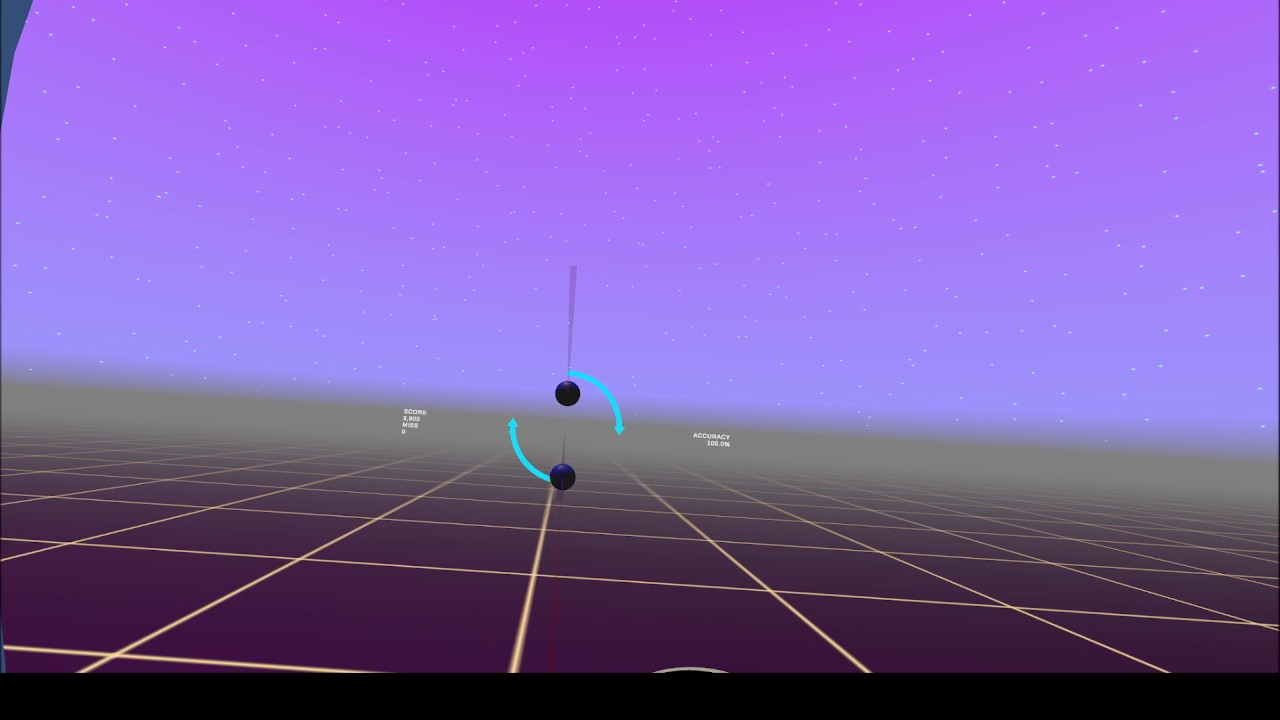
\includegraphics[width=\linewidth]{RotateAfter2.jpg}
  \centering{(b) 회전 후}
\end{minipage}
\caption{노트 하강 및 양손 컨트롤러 기반의 트랙 회전 플레이 화면}
\label{fig:play_screen}
\end{figure}

\subsection{일시정지 및 플레이 결과 UI}
게임 플레이 중 메뉴 버튼을 입력하면 인게임 오디오 재생 버퍼가 멈추며 일시정지 화면이 나타난다. 이때 다가오던 모든 노트와 시각 이펙트를 비활성화되며, Song Select 화면이나 메인 화면으로 이동하거나,  게임을 재개할 수 있다. 곡이 완전히 종료되면 사용자의 플레이 기록(총 점수, 최대 콤보, 정확도)을 집계하여 결과 화면에 나타내며, 달성 정확도에 따른 등급이 산출된다. 플레이 결과 화면의 렌더링 모습은 그림 \ref{fig:result_screen}과 같다.

\begin{figure}[!ht]
\centering
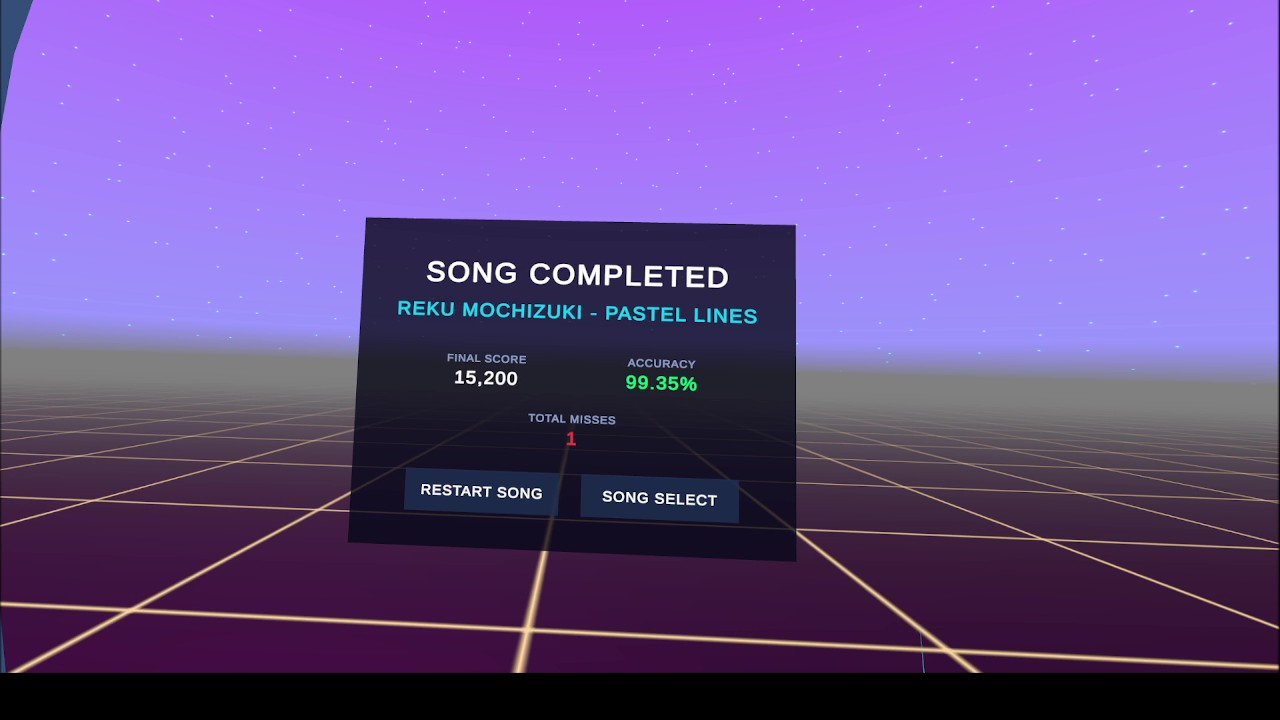
\includegraphics[width=0.85\linewidth]{ResultUI.jpg}
\caption{총 점수 및 정확도 분석 결과 출력 화면(ResultUI)}
\label{fig:result_screen}
\end{figure}

\subsection{웹 기반 채보 에디터 인터페이스}
개발자가 게임 플레이를 위한 채보를 직접 제작하고 관리할 수 있도록 웹 채보 에디터(\texttt{BeatmapEditor.html})를 AI를 이용하여 개발하였다.해당 에디터는 로컬 음악 파일을 업로드하여 타임라인 상에서 음악 재생과 동시에 키보드 단축키 및 마우스 드래그를 활용해 직관적으로 노트를 비트 단위로 배치할 수 있도록 설계되었다. 에디터의 주요 사용자 인터페이스 구동 화면은 그림 \ref{fig:beatmap_editor}와 같다.

\begin{figure}[!ht]
\centering
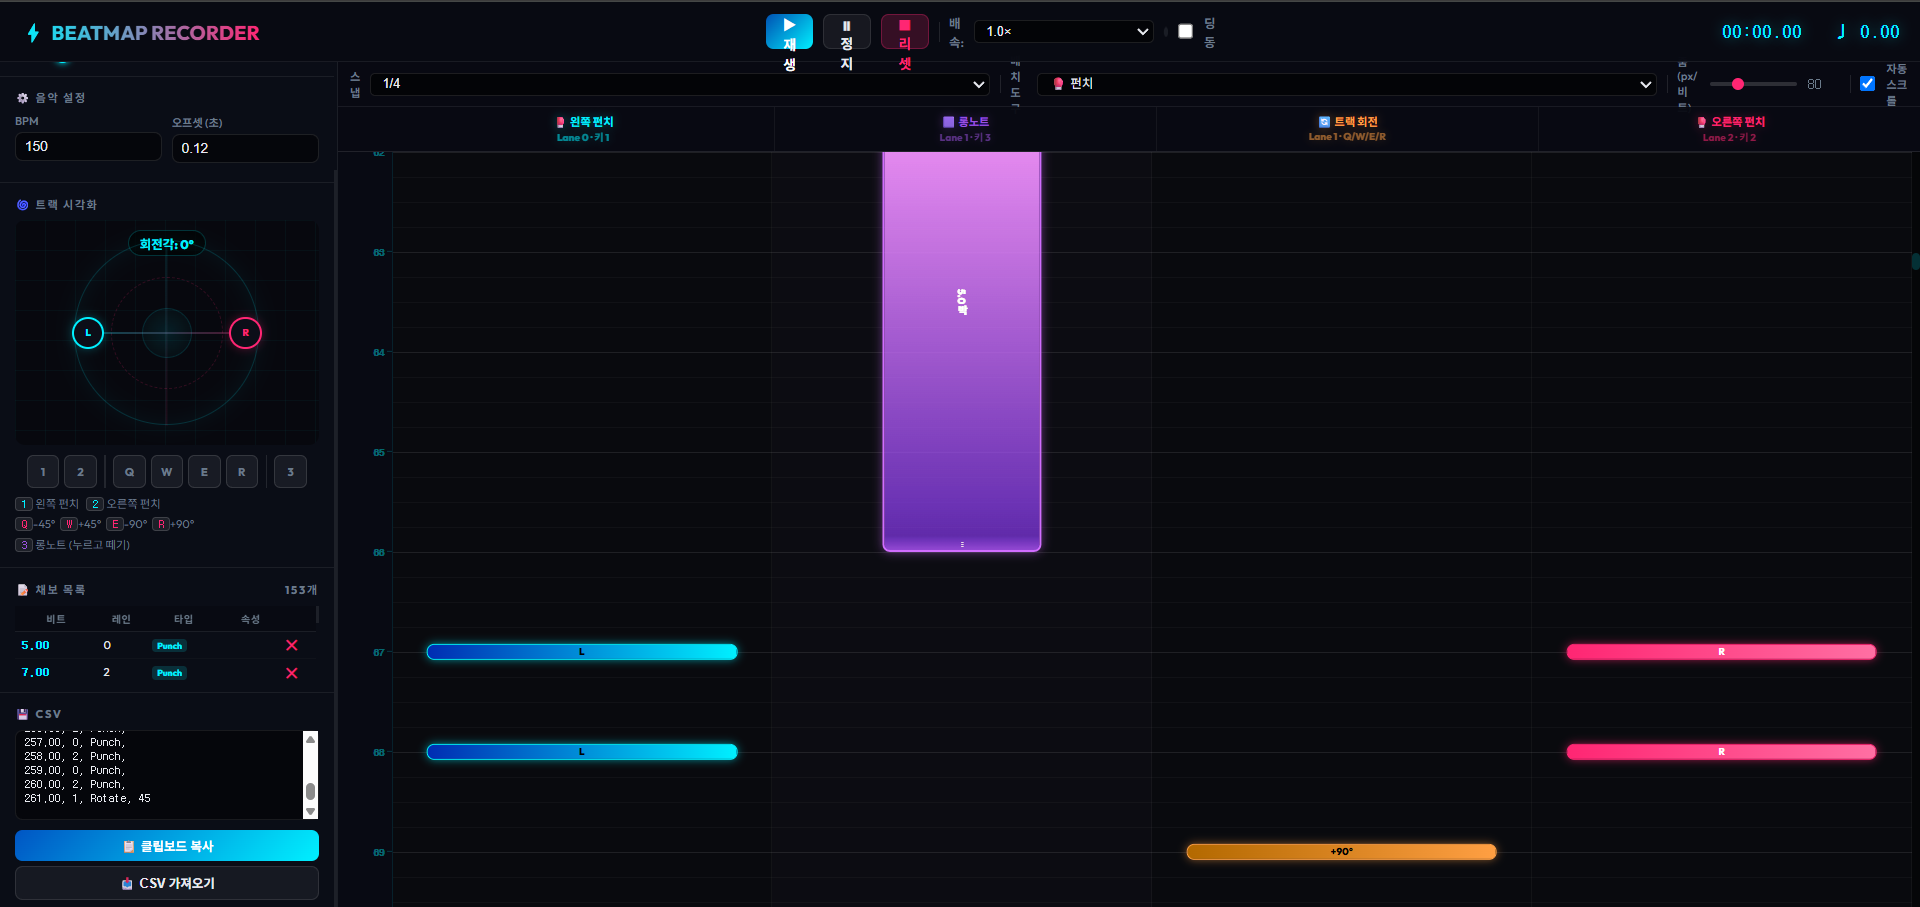
\includegraphics[width=0.85\linewidth]{BeatMapEditor.png}
\caption{BeatmapEditor UI 화면}
\label{fig:beatmap_editor}
\end{figure}


\section{결론 및 향후 과제}
본 연구는 메타버스의 핵심 기술 중 하나인 촉각 피드백을 리듬게임 장르에 접목하여, 실시간 음원 분석 데이터와 Delta 및 Contrast 알고리즘을 기반으로 한 오디오-햅틱 인터랙션 리듬게임 시스템을 구현하였다. 오디오 신호의 FFT 분석 결과를 햅틱 모터 매핑과 결합하여 햅틱 슈트의 전후면 공간 매핑 시스템을 설계하였으며, 이를 컨트롤러의 주파수 대역별 진동으로 이식하여 시각 및 촉각의 감각적 몰입감을 높였다.

또한, 컨트롤러의 위치 차이를 이용한 트랙 회전 메커니즘과 시선 기준 사용자 캘리브레이션 시스템을 구현하여 플레이어의 조작 재미를 높이고 UX를 향상시켰다. 구동 결과, Scene 매니지먼트 구조와 사용자 UI가 유기적으로 연동되어 안정적인 가상현실 리듬게임 환경이 구현되었음을 확인하였다.

다만, 하드웨어 호환성과 테스트 장비 한계로 인해 햅틱 슈트와의 실시간 무선 연동을 직접 검증하는 데는 아쉬움이 남았다. 대신 이를 보완하기 위해 원래 슈트용으로 설계했던 실시간 전후면 진동 제어 로직을 가상현실 컨트롤러의 좌우 진동 피드백으로 이식하여 시스템의 성능을 확인할 수 있었다.

향후에는 주파수 분석 알고리즘을 개선하여 진동 피드백의 깊이감을 더욱 섬세하게 표현하고, 무선 통신 연동을 완료하여 당초 목표했던 전신 햅틱 슈트 피드백을 실제로 구현할 계획이다. 아울러 웹 기반 채보 에디터의 편의성을 개선하고 채보 생성 기능을 최적화하여, 더 다양한 음원과 채보를 제작하고,플랫폼에 배포하는 것을 목표로 작업을 지속적으로 진행할 예정이다.

\end{document}
